Consider a block released from rest on a fixed inclined plane. Gravity tends
to pull it downhill, while friction may slow the descent or prevent motion
altogether. This example connects Newton's second law, double integration,
and the work--energy theorem.

\section{Geometry and assumptions}
Let the plane make an angle $\theta$ with the horizontal, and let $s$ measure
distance down the plane from the release point. The available ramp length is
$L$. The block has mass $m$, and the gravitational acceleration is $g$.
We neglect rotation, air resistance, and deformation of the ramp.
The coefficients of static and kinetic friction satisfy
$0\leq\mu_k\leq\mu_s$.

\begin{center}
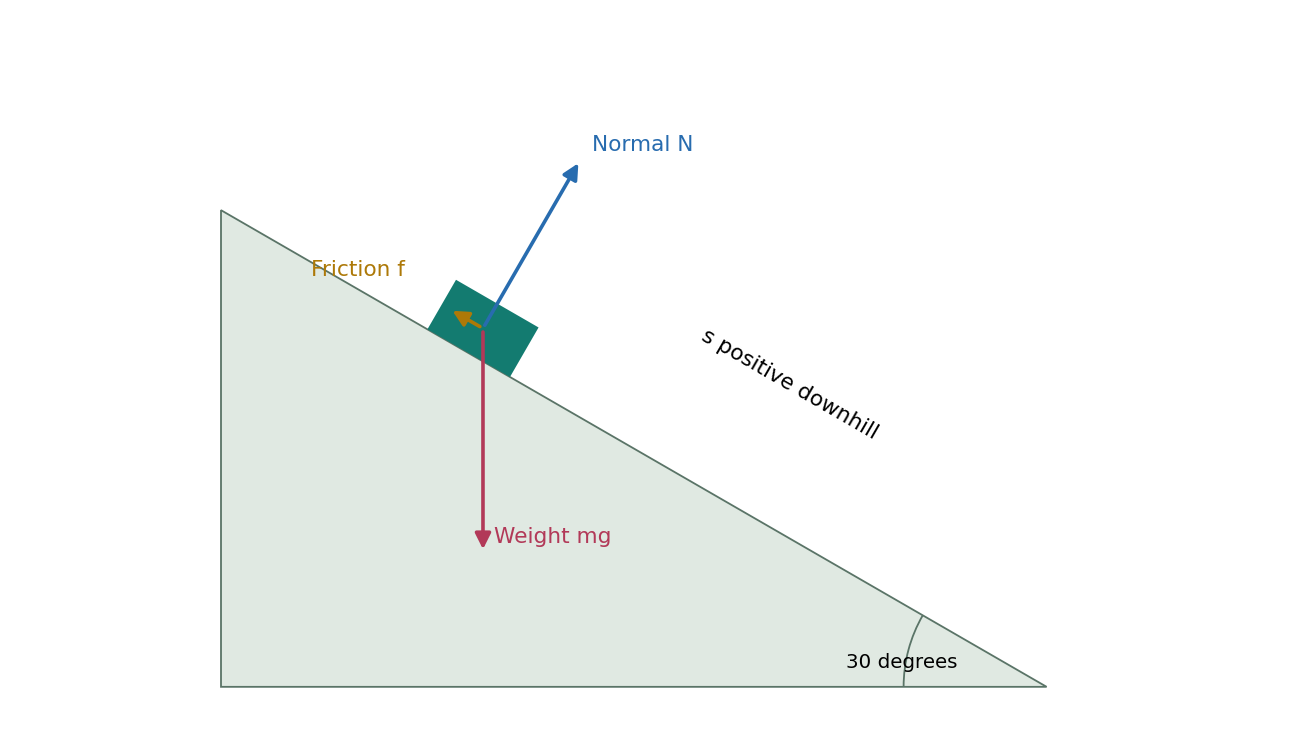
\includegraphics[width=0.95\linewidth]{inclined-plane-forces.png}
\end{center}
The diagram shows the sliding case. The weight $mg$ is vertical, the normal
reaction $N$ is perpendicular to the plane, and friction $f$ points uphill.
The force arrows use a common scale; the block size is illustrative.

\section{Resolve the forces first}
There is no acceleration perpendicular to the plane, so
\begin{equation}
N-mg\cos\theta=0,\qquad N=mg\cos\theta.
\end{equation}
Along the plane, Newton's second law gives
\begin{equation}
m\ddot{s}=mg\sin\theta-f.
\end{equation}
The two components $mg\sin\theta$ and $mg\cos\theta$ are projections of the
single gravitational force, not additional forces to add to $mg$.

\subsection{Will a block released from rest move?}
Static friction can take any required magnitude up to $\mu_s N$. Thus rest
is possible when
\begin{equation}
mg\sin\theta\leq\mu_s mg\cos\theta,
\qquad\hbox{or}\qquad \tan\theta\leq\mu_s.
\end{equation}
In this case $f_s=mg\sin\theta$, $s=0$, and $v=0$. In particular, static
friction is not always equal to $\mu_s N$. Equality is the limiting case;
this idealized release model retains rest at equality.

\subsection{Sliding downhill}
When $\tan\theta>\mu_s$, the static limit is exceeded. Once sliding begins,
$f_k=\mu_k N$, and the constant downhill acceleration is
\begin{equation}
a=g(\sin\theta-\mu_k\cos\theta).
\end{equation}
For the assumed coefficient ordering, a block that starts sliding in this
way has $a>0$. Mass cancels, but the forces and energies still depend on mass.
These equations describe downhill sliding; an initially uphill-moving block
would require reversing the friction direction until it stops.

\section{Integrate twice and impose the initial conditions}
For a constant acceleration, start with $dv/dt=a$. Definite integration
from the initial time $t_0$ gives
\begin{equation}
\int_{v_0}^{v(t)}du=\int_{t_0}^{t}a\,d\tau,
\qquad v(t)=v_0+a(t-t_0).
\end{equation}
Next integrate $ds/dt=v(t)$:
\begin{equation}
s(t)-s_0=\int_{t_0}^{t}\bigl[v_0+a(\tau-t_0)\bigr]d\tau,
\end{equation}
so that
\begin{equation}
s(t)=s_0+v_0(t-t_0)+\frac12 a(t-t_0)^2.
\end{equation}
Equivalently, indefinite integration gives $v=at+C_1$ and
$s=\tfrac12at^2+C_1t+C_2$. The conditions $v(t_0)=v_0$ and $s(t_0)=s_0$
fix $C_1=v_0-at_0$ and $C_2=s_0-v_0t_0+\tfrac12at_0^2$.
The integration constants encode the initial state; they are not extra forces.

Here $t_0=s_0=v_0=0$. The sliding solutions reduce to
\begin{equation}
v(t)=at,\qquad s(t)=\frac12at^2.
\end{equation}
At the ramp foot $s=L$, hence
\begin{equation}
t_{\mathrm{end}}=\sqrt{\frac{2L}{a}},\qquad
v_{\mathrm{end}}=\sqrt{2aL}.
\end{equation}
These arrival formulas require $a>0$ and do not apply to the stationary case.
The calculation ends at arrival, without modeling an impact or a transition
to another surface.

\section{Three worked cases}
Use $m=2\,\mathrm{kg}$, $g=9.81\,\mathrm{m/s^2}$,
$\theta=30^\circ$, and $L=10\,\mathrm{m}$. Then
$mg\sin\theta=9.81\,\mathrm{N}$ and $N\simeq16.9914\,\mathrm{N}$.
\begin{enumerate}
\item Frictionless: $\mu_s=\mu_k=0$. The acceleration is
$4.905\,\mathrm{m/s^2}$; arrival occurs at approximately $2.0193\,\mathrm{s}$
with speed $9.9045\,\mathrm{m/s}$.
\item Sliding with friction: $\mu_s=0.3$, $\mu_k=0.2$.
Since $\tan30^\circ\simeq0.5774>0.3$, the block moves. Kinetic friction is
approximately $3.3983\,\mathrm{N}$, giving $a\simeq3.2059\,\mathrm{m/s^2}$,
$t_{\mathrm{end}}\simeq2.4977\,\mathrm{s}$, and
$v_{\mathrm{end}}\simeq8.0073\,\mathrm{m/s}$.
\item Held by static friction: $\mu_s=0.7$, $\mu_k=0.5$.
The static limit is approximately $11.8940\,\mathrm{N}$, but only
$9.81\,\mathrm{N}$ is needed. The block remains at rest.
\end{enumerate}

\section{Check the energy balance}
Choose zero gravitational potential at the foot of the ramp. At distance $s$,
\begin{equation}
K=\frac12mv^2,\qquad U=mg(L-s)\sin\theta,\qquad Q=f_k s
\end{equation}
for the sliding cases. Here $Q$ is mechanical energy dissipated at the contact,
not heat assigned solely to the block. The work--energy theorem gives
\begin{equation}
\frac12mv^2=(mg\sin\theta-f_k)s,
\qquad K+U+Q=mgL\sin\theta=98.1\,\mathrm{J}.
\end{equation}
Without friction, all initial potential energy becomes kinetic energy.
With $\mu_k=0.2$, about $33.983\,\mathrm{J}$ is dissipated and
$64.117\,\mathrm{J}$ becomes kinetic energy by arrival. In static equilibrium
there is no displacement, no frictional work, and no mechanical energy loss.

\section{Computational resource}
The accompanying Julia project evaluates the augmented state
$\boldsymbol{u}=(s,v,1)^{\mathsf T}$ using
\begin{equation}
\dot{\boldsymbol{u}}=A\boldsymbol{u},\qquad
A=\begin{pmatrix}0&1&0\\0&0&a\\0&0&0\end{pmatrix},\qquad
\boldsymbol{u}(t)=\exp(tA)\boldsymbol{u}(0).
\end{equation}
The third component supplies the constant forcing. Independent checks use
the integrated formulas above, the arrival condition, and energy conservation.
Each case contains 181 samples. Moving cases are sampled up to arrival;
the stationary case is sampled for four seconds.

\begin{center}

\includegraphics[width=0.95\linewidth]{comparison.png}
\end{center}
The \PMlinkexternal{inclined-plane explorer}{https://images.physicslibrary.org/examples/inclined-plane/index.html}
shows the saved trajectories with an animated block and force vectors.
The Julia source, environment, CSV data, and offline explorer are downloadable.

\section{Questions to explore}
\begin{enumerate}
\item Why does doubling the mass leave the arrival time unchanged but double
the normal force and dissipated energy?
\item What is the critical release angle for a material with $\mu_s=0.7$?
\item How does setting $\mu_k=0$ recover the frictionless solution?
\item Why does applying $f=\mu_sN$ to every stationary block give an incorrect
force balance?
\end{enumerate}
